\section{Experiments}
\label{sec:xp}

This Section presents some experiments obtained with the previously described method.

\subsection{Training the neural networks}

The DNN proposed in the Figure~\ref{fig:nn} was trained
on the DSD100 dataset.
First at all, STFT features were computed. With an hop size of $1024$ samples,
around 180k samples were computed. Samples were then grouped into batches of 256 samples.
After each batch, the model was optimized according to the mean square error.
The Figure~\ref{fig:train-basic} shows the accuracy of the model over a few epochs.
Accuracy is compared with the validation set to detect whether the model is
over-fitting or not.

\begin{figure}
  \centering
  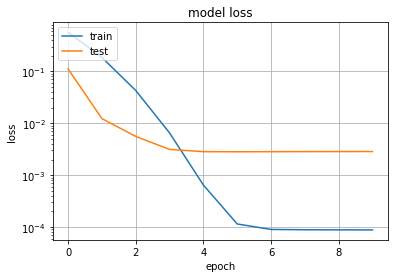
\includegraphics[width=0.8\columnwidth]{train-basic.png}
  \label{fig:train-basic}
  \caption{Loss during the training}
\end{figure}

\subsection{Improving the model}

It appears that the network was completely overfitting. Overfitting might be induced
by a few factors: the high number of parameters, the correlation between the input
features, the heavy pre-processing steps.

\begin{figure}
  \centering
  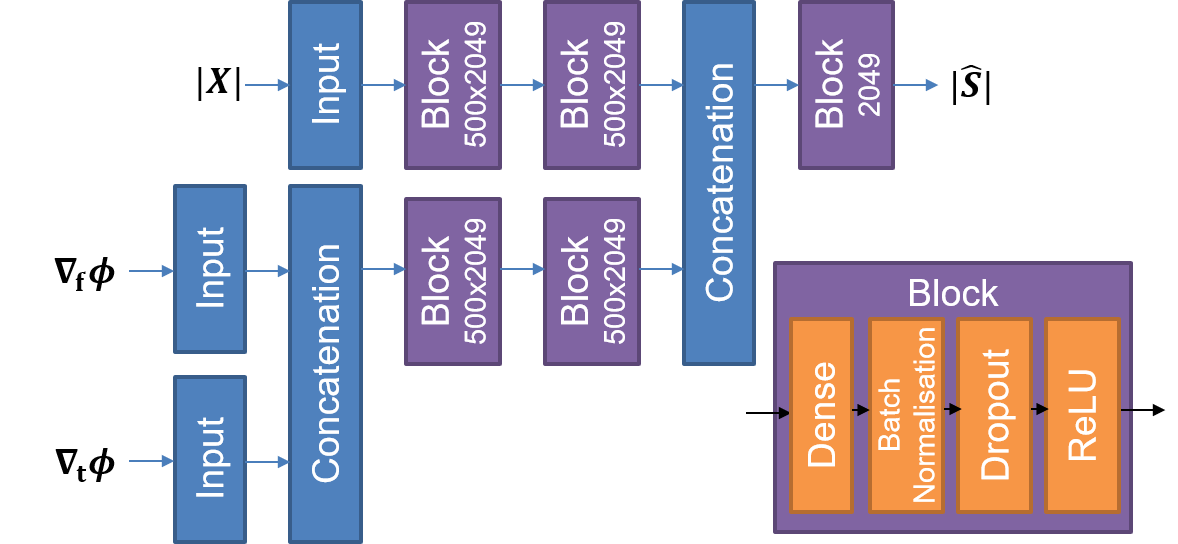
\includegraphics[width=0.9\columnwidth]{final-architecture.png}
  \label{fig:final-architecture}
  \caption{Improvements of the neural network}
\end{figure}

Consequently, I brought some changes to the neural network, as shown in Figure
\ref{fig:final-architecture}. The dense layers and the activation functions are
replaced by blocks containing a dense layer, a batch normalization layer,
 a dropout layer and an activation function.
The dense layers are using multi-channels, such that
the number of parameters were narrowed down to around 550k.
The Figure~\ref{fig:train-final} shows the training loss of the new model.
A significant improvement was obtained.

\begin{figure}
  \centering
  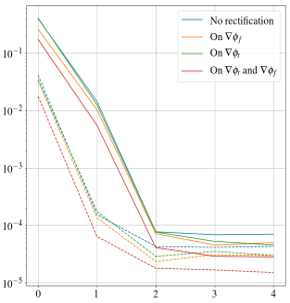
\includegraphics[width=0.6\columnwidth]{train-final.png}
  \label{fig:train-final}
  \caption{Loss during the training after the improvement of the network}
\end{figure}

\subsection{Signal to distortion ratio}

Literature is commonly using 3 metrics, SDR (signal to distortion ratio),
SIR (signal to interferences ratio) and SAR (signal to artifacts ratio).
Errors in source separation might come from two origins:
noise due to mis-separation, called interferences, and noise to the reconstruction
algorithm itself, called crosstalk.
%Typically, increasing the STFT window size tends to increase SIR, but decrease SAR.
The Table~\ref{tab:res} presents the metrics SDR for the case with the original
neural network, the final architecture with and without the correction
of the feature distributions.
The methods "LSTM" and "WaveNet" are presented in the Section~\ref{sec:related}.

\begin{table}
  \centering
  \begin{tabular}{|c| c c c c| }
  \hline
    Sources & Vocal & Bass & Drums & Other \\
  \hline
    Original & 2.32 & 1.01 & 1.39 & 1.32 \\
  \hline
    No rectification & 3.48 & 2.15 & 2.71 & 2.O1 \\
  \hline
    Rectified distributions & 3.51 & 2.10 & 2.72 & 2.12 \\
  \hline
    WaveNet & 4.60 & 2.49 & 4.60 & 0.54 \\
  \hline
    LSTM & 6.31 & 3.73 & 5.46 & 4.33 \\
  \hline
  \end{tabular}
  \label{tab:res}
    \caption{Signal to distortion ratio for the method proposed in the report compared with state-of-the-art methods}
\end{table}


\subsection{Analysis of a result}

\begin{figure}
  \centering
  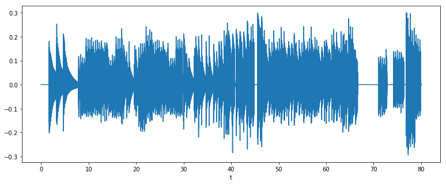
\includegraphics[width=0.8\columnwidth]{bass-src.png}
  \label{fig:bass-src}
  \caption{Source signal of the bass}

  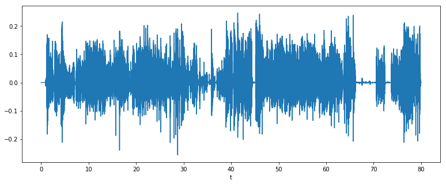
\includegraphics[width=0.8\columnwidth]{bass-pred.png}
  \label{fig:bass-pred}
  \caption{Source signal of the prediction}
\end{figure}

For one example song, the Figure~\ref{fig:bass-src} presents the bass source,
whereas the Figure~\ref{fig:bass-pred} shows the prediction source.
We can observe that long patterns such as fading at the beginning are not learned.
One explanation is that the time context is too short for these patterns.
Furthermore, the neural network tends to empty gaps, creating a feeling of
a white noise.

I tried to compute the source "Other" as the difference between the signal of
the mixture and the other source signals, but it provides a very distorted signal.
This shows that errors in other source signals remain significant.
